%%% fs-seim-intro - Introduction

\label {fs-intro}

Nowadays, a lot of real-life applications use stream processing for network monitoring, financial analysis, training machine learning models, etc. State-of-the-art industrial stream processing systems, such as Flink \cite{carbone2015apache}, Samza \cite{Noghabi:2017:SSS:3137765.3137770}, Storm \cite{apache:storm}, Heron \cite{Kulkarni:2015:THS:2723372.2742788}, are able to provide low-latency and high-throughput in distributed environment for a wide range of analytical problems. However, issues related to the order-sensitive computations still remain. Most of these systems assume that events are fed to the system with monotonically increasing timestamps or with minor inversions. Often, such timestamps can be assigned at system's entry. Nevertheless, even if input items arrive at system's entry monotonically, they can be reordered because of parallel and asynchronous processing. In this case, order-sensitive operations located in data flow pipeline quite deeply can be broken. Figure ~\ref{break-order-dataflow} shows the example of common distributed stream processing pipeline that breaks the input order of operation, even if input events are monotonic and links between operations guarantee FIFO order. Basically, ordering constraints make sense only for stateful operations.

\begin{figure}[htbp]
  \centering
  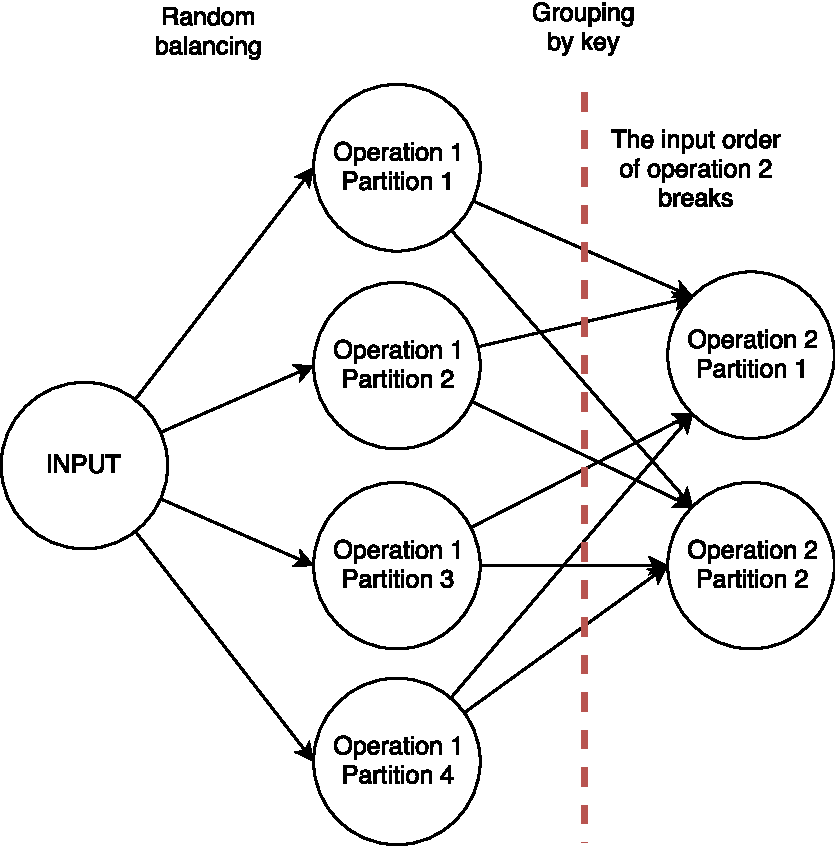
\includegraphics[width=0.38\textwidth]{pics/break_order_pipeline}
  \caption{An  example of common distributed stream processing pipeline that breaks the input order of operation}
  \label {break-order-dataflow}
\end{figure}

The typical way to achieve in-order processing is to buffer operation's input for some time to ensure that there are no out-of-order items. Most of the modern stream processing systems provide functionality to buffer all input items before specified operations until some user-provided conditions are satisfied. Conditions can be set on timing or the count of elements in the buffer. The main disadvantage of such techniques is that it can lead to significantly large latency, especially if the processing pipeline contains several operations that require ordered input. 

An alternative option is to handle out-of-order items as a special case in the business logic of operation. However, this way is suitable only for the limited number of tasks. Moreover, it may dramatically complicate the business-logic, which can lead to increasing the cost of its maintenance and is error-prone.
% sophisticated bugs.    

In this paper, we propose an optimistic approach to handle out-of-order events in any stateful operation. In addition, we demonstrate its advantages compared to existing solutions. The contributions of this paper are the following: 

\begin {itemize}
\item Definition of new optimistic technique to handle out-of-order items in stateful operations
\item Demonstration of properties of this approach
\item Demonstration of working example that applies proposed method
\end {itemize}

The rest of the paper is structured as follows: in section~\ref{fs-stream} we formalize the preliminaries of stream processing, the examples of tasks that require ordered input are described in section~\ref{fs-tasks}, the typical approaches for handling out-of-order events are discussed in~\ref{fs-typical}, our optimistic technique is detailed in~\ref{fs-optimistic} and its performance is demonstrated in ~\ref{fs-experiments}, the main differences between proposed method and existing ones are shown in~\ref{fs-related}, finally we discuss the results and our plans in~\ref{fs-conclusion}.
